% Template adapted from https://github.com/jgm/pandoc-templates/blob/master/default.latex
% To be used with XeLaTex in memoiR
%%%%%%%%%%%%%%%%%%%%%%%%%%%%%%%%%%%%%%%%%%%%%%%%%%%%%%%%%%%%%%%%%%%%%%%%%%%%%%%%%%%%%%%%%

% Options for packages loaded elsewhere
\PassOptionsToPackage{unicode=true}{hyperref}
\PassOptionsToPackage{hyphens}{url}
\PassOptionsToPackage{dvipsnames,svgnames*,x11names*}{xcolor}
% Right to left support


\documentclass[
  9pt,
  american,
  a5paper,
  extrafontsizes,onecolumn,openright
  ]{memoir}

% Double (or whatever) spacing

% Math
\usepackage{amssymb, amsmath}
% mathspec: arbitrary math fonts
\usepackage{unicode-math}
\defaultfontfeatures{Scale=MatchLowercase}
\defaultfontfeatures[\rmfamily]{Ligatures=TeX,Scale=1}

% Fonts
\usepackage{lmodern}
\usepackage{fontspec}
% Main font
% Specific sanserif font
% Specific monotype font
% Specific math font
% Chinese, Japanese, Corean fonts

% Use upquote for straight quotes in verbatim environments
\usepackage{upquote}
% Use microtype
\usepackage[]{microtype}
\UseMicrotypeSet[protrusion]{basicmath} % disable protrusion for tt fonts

% Verbatim in note

% Color links
\usepackage{xcolor}

% Strikeout

% Necessary for code chunks

% Listings package

% Tables
\usepackage{longtable,booktabs,tabu}
% Fix footnotes in tables (requires footnote package)
\IfFileExists{footnote.sty}{\usepackage{footnote}\makesavenoteenv{longtable}}{}

% Graphics
\usepackage{graphicx,grffile}
\graphicspath{{images/}}
\makeatletter
\def\maxwidth{\ifdim\Gin@nat@width>\linewidth\linewidth\else\Gin@nat@width\fi}
\def\maxheight{\ifdim\Gin@nat@height>\textheight\textheight\else\Gin@nat@height\fi}
\makeatother
% Scale images if necessary, so that they will not overflow the page
% margins by default, and it is still possible to overwrite the defaults
% using explicit options in \includegraphics[width, height, ...]{}
\setkeys{Gin}{width=\maxwidth,height=\maxheight,keepaspectratio}

% Custom figure captions
\usepackage{caption}
\captionsetup[figure]{labelfont=bf, labelsep=period, font=small}

% Prevent overfull lines
\setlength{\emergencystretch}{3em}  
\providecommand{\tightlist}{%
  \setlength{\itemsep}{0pt}\setlength{\parskip}{0pt}}

% Number sections for memoir (secnumdepth counter is ignored)
\setsecnumdepth{section}

% Set default figure placement to htbp
\makeatletter
\def\fps@figure{htbp}
\makeatother

% Spacing in lists
\usepackage{enumitem}

% Polyglossia
\usepackage{polyglossia}
\setmainlanguage{en-US}

% localized quotes
\usepackage[strict,autostyle]{csquotes}

% BibLaTeX
\usepackage[backend=biber,style=authoryear-ibid,isbn=false,backref=true,giveninits=true,uniquename=init,maxcitenames=2,maxbibnames=150,sorting=nyt,sortcites=false]{biblatex}
\addbibresource{references.bib}

% cslreferences environment required by pandoc > 2.7



%%%%%%%%%%%%%%%%%%%%%%%%%%%%%%%%%%%%%%%%%%%%%%%%%%%%%%%%%%
% memoiR format

% Chapter Summary environment 
\usepackage[tikz]{bclogo}
\newenvironment{Summary}
  {\begin{bclogo}[logo=\bctrombone, noborder=true, couleur=lightgray!50]{}\parindent0pt}
  {\end{bclogo}}
% Syntax:
%
%```{block, type='Summary'}
% Deliver message here.
% ```

% scriptsize code 
\let\oldverbatim\verbatim
\def\verbatim{\oldverbatim\scriptsize}
% Applies to code blocks and R code results
% code chunk options size='scriptsize' applies only to R code and results
% if the code chunk sets a different size, \def\verbatim{...} is prioritary for code results 


% memoiR dalef3 chapter style 
% https://ctan.crest.fr/tex-archive/info/latex-samples/MemoirChapStyles/MemoirChapStyles.pdf
\usepackage{soul}
\definecolor{nicered}{rgb}{0.247, 0.0, 0.490}
\makeatletter
\newlength\dlf@normtxtw
\setlength\dlf@normtxtw{\textwidth}
\def\myhelvetfont{\def\sfdefault{mdput}}
\newsavebox{\feline@chapter}
\newcommand\feline@chapter@marker[1][4cm]{%
  \sbox\feline@chapter{%
    \resizebox{!}{#1}{\fboxsep=1pt%
	  \colorbox{nicered}{\color{white}\bfseries\sffamily\thechapter}%
	}}%
  \rotatebox{90}{%
    \resizebox{%
	  \heightof{\usebox{\feline@chapter}}+\depthof{\usebox{\feline@chapter}}}%
	{!}{\scshape\so\@chapapp}}\quad%
  \raisebox{\depthof{\usebox{\feline@chapter}}}{\usebox{\feline@chapter}}%
 }
\newcommand\feline@chm[1][4cm]{%
  \sbox\feline@chapter{\feline@chapter@marker[#1]}%
  \makebox[0pt][l]{% aka \rlap
    \makebox[1cm][r]{\usebox\feline@chapter}%
  }}
\makechapterstyle{daleif1}{
  \renewcommand\chapnamefont{\normalfont\Large\scshape\raggedleft\so}
  \renewcommand\chaptitlefont{\normalfont\huge\bfseries\scshape\color{nicered}}
  \renewcommand\chapternamenum{}
  \renewcommand\printchaptername{}
  \renewcommand\printchapternum{\null\hfill\feline@chm[2.5cm]\par}
  \renewcommand\afterchapternum{\par\vskip\midchapskip}
  \renewcommand\printchaptertitle[1]{\chaptitlefont\raggedleft ##1\par}
}
\makeatother


% Layout
%%%%%%%%%%%%%%%%%%%%%%%%%%%%%%%%%%%%%%%%%%%%%%%%%%%%%%%%%%

% Based on memoir, style companion
\newcommand{\MemoirChapStyle}{daleif1}
\newcommand{\MemoirPageStyle}{Ruled}

% Space between paragraphs
\usepackage{parskip}
  \abnormalparskip{3pt}

% Adjust margin paragraphs vertical position
\usepackage{marginfix}


% Margins
%%%%%%%%%%%%%%%%%%%%%%%%%%%%%%%%%%%%%%%

% allow use of '-',+','/' ans '*' to make simple length computation
\usepackage{calc}

% Full-width figures utilities
\newlength\widthw % full width
\newlength{\rf}
\newcommand*{\definesHSpace}{
  \strictpagecheck % slower but efficient detection of odd/even pages
  \checkoddpage
  \ifoddpage
  \setlength{\rf}{0mm}
  \else
  \setlength{\rf}{\marginparsep+\marginparwidth}
  \fi
}

\makeatletter
% 1" margins for the front matter.
\newcommand*{\SmallMargins}{
  \setlrmarginsandblock{0.75in}{0.75in}{*}
  \setmarginnotes{0.1in}{0.1in}{0.1in}
 \setulmarginsandblock{0.75in}{0.75in}{*}
  \checkandfixthelayout
  \ch@ngetext
  \clearpage
  \setlength{\widthw}{\textwidth+\marginparsep+\marginparwidth}
  \footnotesatfoot
  \chapterstyle{\MemoirChapStyle}  % Chapter and page styles must be recalled
  \pagestyle{\MemoirPageStyle}
}

% 3" outer margin for the main matter
\newcommand{\LargeMargins}{\SmallMargins}
\makeatother

% Figure captions and footnotes in outer margins


% Local toc
%%%%%%%%%%%%%%%%%%%%%%%%%%%%%%%%%%%%%%%%%%%%%%%%%%%%%%%%%%

\usepackage{titletoc}
\newcommand{\toc}[1]{%
  \startcontents[chapters]%
  \printcontents[chapters]{}{1}[#1]{}%
  ~\newline%
}


% Text boxes
%%%%%%%%%%%%%%%%%%%%%%%%%%%%%%%%%%%%%%%%%%%%%%%%%%%%%%%%%%

% Define a style for mdframed boxes
\mdfdefinestyle{boxstyle}{
	skipabove=1.5\topskip,
	skipbelow=.5\topskip,
	rightmargin=0pt,
	leftmargin=0pt,
	innerrightmargin=7pt,
	innerleftmargin=7pt,
	topline=false,
	bottomline=false,
	rightline=false,
	leftline=false,
	frametitlerule=true,
	linecolor=black,
	fontcolor=black,
	frametitlealignment=\noindent
}


% Main title page with filigrane
%%%%%%%%%%%%%%%%%%%%%%%%%%%%%%%%%%%%%%%%%%%%%%%%%%%%%%%%%%

% Text blocks
\usepackage[absolute,overlay]{textpos}
  \setlength{\TPHorizModule}{1mm}
  \setlength{\TPVertModule}{1mm}

\newcommand{\MainTitlePage}[2]{
  \SmallMargins % Margins
  \pagestyle{empty} % No header/footer
  \textblockorigin{\stockwidth-\paperwidth-\trimedge}{\trimtop} % recto
  \begin{textblock*}{2mm}(\spinemargin/2,\uppermargin/2)
    \rule{1pt}{\paperheight-\uppermargin}
  \end{textblock*}
  \begin{textblock*}{\paperwidth*2/3}(\paperwidth/5, \paperheight/5)
    \flushright
    \begin{Spacing}{3}
      {\fontfamily{qtm}\selectfont\fontsize{45}{45}\selectfont\textsc{\thetitle}}
    \end{Spacing}
  \end{textblock*}
    \begin{textblock*}{\paperwidth*2/3}(\paperwidth/5, \paperheight/2)
    \flushright
    {\fontfamily{qtm}\huge\theauthor}
  \end{textblock*}
    \begin{textblock*}{\paperwidth*2/3}[0, 1](\spinemargin, \uppermargin+\textheight)
    \normalfont\thedate
  \end{textblock*}
  ~\\ % Print a character or the page will not exist
  \newpage
  \textblockorigin{\trimedge}{\trimtop} % verso
  \begin{textblock*}{\textwidth}(\paperwidth-\spinemargin-\textwidth, \uppermargin)
    #1
  \end{textblock*}
  \begin{textblock*}{\textwidth}[0,1](\paperwidth-\spinemargin-\textwidth, \uppermargin+\textheight+\footskip)
    \centering
          \includegraphics[width=\paperwidth/4]{logo}\\ \bigskip
        #2
  \end{textblock*}
  ~\\ % Print a character or the page will not exist
  \newpage
}

% Clear page and open an even one (\clearpage opens an odd one)
\newcommand{\evenpage}{
  \clearpage
  \strictpagecheck % slower but efficient detection of odd/even pages
  \checkoddpage
  \ifoddpage
    \thispagestyle{empty}
    ~\\ % Print a character or the page will not exist
    \newpage
  \else
    % do nothing
  \fi
}


%% PDF title page to insert
%%%%%%%%%%%%%%%%%%%%%%%%%%%%%%%%%%%%%%%%%%%%%%%%%%%%%%%%%%



%% Bibliography
%%%%%%%%%%%%%%%%%%%%%%%%%%%%%%%%%%%%%%%%%%%%%%%%%%%%%%%%%%

% Repeated citation as author-year-title instead of author-title (modification of footcite:note in verbose-inote.cbx)

%% Table of Contents
%%%%%%%%%%%%%%%%%%%%%%%%%%%%%%%%%%%%%%%%%%%%%%%%%%%%%%%%%%

% fix the typesetting of the part number
\renewcommand\partnumberlinebox[2]{#2\ ---\ }


% Fonts
%%%%%%%%%%%%%%%%%%%%%%%%%%%%%%%%%%%%%%%%%%%%%%%%%%%%%%%%%%


% Hyperref comes last
%%%%%%%%%%%%%%%%%%%%%%%%%%%%%%%%%%%%%%%%%%%%%%%%%%%%%%%%%%

\usepackage{hyperref}
\hypersetup{
  pdftitle={The Dismutators},
  pdfauthor={Daniel Moreira},
  colorlinks=true,
  linkcolor=Purple,
  citecolor=Blue,
  urlcolor=blue,
  breaklinks=true}

% Don't use monospace font for urls
\urlstyle{same}


% Title, author, date from YAML to LaTeX
%%%%%%%%%%%%%%%%%%%%%%%%%%%%%%%%%%%%%%%%%%%%%%%%%%%%%%%%%%

\title{The Dismutators}

\author{Daniel Moreira}

\date{}


% Include headers (preamble.tex) here
%%%%%%%%%%%%%%%%%%%%%%%%%%%%%%%%%%%%%%%%%%%%%%%%%%%%%%%%%%
% Add LaTeX code into the preamble of the document here
\hyphenation{bio-di-ver-si-ty sap-lings}

% Define colors for text boxes
\definecolor{grey}{HTML}{F5F5F5}

% Define text box environments
\newmdenv[
	style=boxstyle,
	backgroundcolor=grey,
	frametitlebackgroundcolor=grey,
]{greybox}
\usepackage{booktabs}
\usepackage{longtable}
\usepackage{array}
\usepackage{multirow}
\usepackage{wrapfig}
\usepackage{float}
\usepackage{colortbl}
\usepackage{pdflscape}
\usepackage{tabu}
\usepackage{threeparttable}
\usepackage{threeparttablex}
\usepackage[normalem]{ulem}
\usepackage{makecell}
\usepackage{xcolor}


% End of preamble
%%%%%%%%%%%%%%%%%%%%%%%%%%%%%%%%%%%%%%%%%%%%%%%%%%%%%%%%%%


\begin{document}
\frontmatter

% Title page
%%%%%%%%%%%%%%%%%%%%%%%%%%%%%%%%%%%%%%%%%%%%%%%%%%%%%%%%%%


\MainTitlePage{``How have living systems, which are based on a common set of biochemical structures and
processes and subject to a common set of physical-chemical laws, been able to adapt to
the enormously wide spectrum of environmental conditions found in the biosphere?''
Peter Hochachka and George Somero -- Biochemical Adaptation (2002)}{Daniel Moreira

\url{http://www.mdcscience.com}

More text here.}


% Before Body
%%%%%%%%%%%%%%%%%%%%%%%%%%%%%%%%%%%%%%%%%%%%%%%%%%%%%%%%%%





% Contents
%%%%%%%%%%%%%%%%%%%%%%%%%%%%%%%%%%%%%%%%%%%%%%%%%%%%%%%%%%

\LargeMargins
{
\hypersetup{linkcolor=}
\setcounter{tocdepth}{1}
\tableofcontents
}


% Body
%%%%%%%%%%%%%%%%%%%%%%%%%%%%%%%%%%%%%%%%%%%%%%%%%%%%%%%%%%

\LargeMargins
\scriptsize

\normalsize

\chapter*{Preface to this Book Series}\label{preface-to-this-book-series}
\addcontentsline{toc}{chapter}{Preface to this Book Series}

This is a book series of protocol book of methods to measure the activity of antioxidant enzymes, oxidative stress markers, and other related biochemical variables.

More than a decade of experience

The ideia is that each volume is self-contained. To do so, some basic concepts are repeated in each volume so that the readers does not need to refer to another volume while reading / using in the lab bench a protocol.

So far, the plan is to have the following volumes:

Volume 1 - The Dismutators

\mainmatter

\part{Fundamental Concepts}\label{part-fundamental-concepts}

\chapter{Analytical Chemistry}\label{analytical-chemistry}

\chapter{Terminology}\label{terminology}

\chapter{Spectrophotometry Fundamentals}\label{spectrophotometry-fundamentals}

\begin{Summary}
Some text for this block.

\end{Summary}

\toc{1}

\newpage

\section{Spectrophotometry}\label{spectrophotometry}

Spectroscopic methods are those that rely on the interaction between matter and electromagnetic radiation. They encompasses several techniques used to measure how electromagnetic radiation is absorbed, emitted, or scattered by substances. By investigating these interactions, valuable insights into the composition, structure, and properties of different materials are made available.

Wavelength (\(\lambda\)) is defined as the distance between successive peaks of a wave. It is typically measured in meters (m), centimeters (cm), or nanometers (nm). Wavelength is a crucial parameter in spectroscopy as it determines the energy and type of electromagnetic radiation. The electromagnetic spectrum is classified based on wavelength into different regions, each associated with specific types of electromagnetic radiation:

\begin{itemize}
\tightlist
\item
  \textbf{Gamma Rays}: Wavelengths less than \(0.01 \, \text{nm}\)
\item
  \textbf{X-rays}: Wavelengths between \(0.01 \, \text{nm}\) and \(10 \, \text{nm}\)
\item
  \textbf{Ultraviolet (UV)}: Wavelengths between \(10 \, \text{nm}\) and \(400 \, \text{nm}\)
\item
  \textbf{Visible Light}: Wavelengths between \(400 \, \text{nm}\) and \(700 \, \text{nm}\)
\item
  \textbf{Infrared (IR)}: Wavelengths between \(700 \, \text{nm}\) and \(1 \, \text{mm}\)
\item
  \textbf{Microwaves}: Wavelengths between \(1 \, \text{mm}\) and \(1 \, \text{m}\)
\item
  \textbf{Radio Waves}: Wavelengths greater than \(1 \, \text{m}\)
\end{itemize}

\scriptsize

\begin{figure}

{\centering \includegraphics[width=1\linewidth]{Volume-1_files/figure-latex/fig-electromagnetic-rad-1} 

}

\caption{(ref:fig-electromagnetic-rad)}\label{fig:fig-electromagnetic-rad}
\end{figure}

\normalsize

Different regions of the electromagnetic spectrum are utilized in various spectroscopic techniques based on the type of information required and the nature of the sample being analyzed.

Spectrophotometry is a subset of spectroscopy that focuses on measuring the amount of light absorbed by a sample at specific wavelengths. This technique is widely used in biology, chemistry, and various other areas of science and industry to quantify the concentration of substances, monitor chemical reactions, and study molecular interactions. Measuring how much light a sample absorbs (at a given or a set of wavelengths) provides qualitative and quantitative information. The amount of light absorbed by a sample is quantified as absorbance, which is defined as the \enquote{logarithm of the ratio of incident to transmitted radiant power through a sample} \autocite{gold_iupac_2019}.

\subsection{How a Typical Spectrophotometer Functions}\label{how-a-typical-spectrophotometer-functions}

A spectrophotometer is an instrument designed to measure the intensity of light at a given wavelength after its interaction with a sample. A detailed view of spectroscopy and how spectrophotometers work can be found elsewhere \autocite{skoog_fundamentals_2022}. Here is \textbf{a simplified overview} of a typical spectrophotometer, which is enough for the purpose of the protocols in this book:

\begin{itemize}
\item
  \textbf{Light Source}: The spectrophotometer contains a light source, such as a tungsten or xenon lamp, that emits a broad spectrum of light.
\item
  \textbf{Monochromator}: The emitted light is directed into a monochromator, which is a device that separates the light into its component wavelengths. The monochromator can be a prism, a diffraction grating, or a filter. By selecting a specific wavelength, the monochromator ensures that only light of a narrow wavelength band reaches the sample.
\item
  \textbf{Sample Holder}: The light of the selected wavelength passes through the sample holder, which contains the sample to be analyzed. As the light interacts with the sample, some of it is absorbed, and the rest is transmitted or reflected.
\item
  \textbf{Detector}: After passing through the sample, the light reaches a detector. The detector measures the intensity of the transmitted light. The detector converts the light into an electrical signal proportional to the light intensity.
\item
  \textbf{Data Processing}: The electrical signal is then processed and converted into digital data. The spectrophotometer software calculates the absorbance or transmittance of the sample by comparing the intensity of the light before and after it passes through the sample. The absorbance (\(A\)) is calculated as the logarithm (base 10) of the ratio of the initial intensity (\(I_0\)) to the transmitted intensity (\(I\)):
\end{itemize}

\[ A = \log\left(\frac{I_0}{I}\right) \]

\[ A = -\log(T) \]

where \(A\) is absorbance, a measure of the amount of light absorbed by the sample; \(I_0\) is the initial intensity of the light before it passes through the sample; \(I\) is the transmitted intensity of the light after it has passed through the sample; \(T\) is transmittance defined as the ratio \(\frac{I_0}{I}\). This relationship indicates how much light is absorbed by the sample at \textbf{a specific wavelength}.

\begin{greybox}[frametitle = Note]
\emph{Transmittance, the ratio of the transmitted light intensity to the initial light intensity, is dimensionless and is often expressed as a percentage or a fraction is a dimensionless quantity. Despite also being dimensionless, for practical purposes, absorbance is often expressed as absorbance units (AU) and related units such as the milli-absorbance unit (mAU) commonly used in high-performance liquid chromatography with spectrophotometric detectors.}

\end{greybox}

\begin{itemize}
\tightlist
\item
  \textbf{Output}: The final data is displayed on a screen or printed out as a spectrum, which shows the absorbance or transmittance as a function of wavelength. This spectrum provides valuable information about the sample's optical properties and can be used to identify and quantify specific substances within the sample.
\end{itemize}

\section{Lambert-Beer Law}\label{lambert-beer-law}

The Lambert-Beer Law describes the linear relationship between absorbance and the concentration of an absorbing species in a sample. This allows the determination of the concentration of a species based on the absorbance of sample at a given wavelength. The Lambert-Beer Law is expressed by:

\[ A = \varepsilon \cdot C \cdot l \]

where \(A\) is absorbance; \(\varepsilon\) is the molar absorptivity (also known as molar extinction coefficient), a constant that indicates how strongly the absorbing species absorbs light at a particular wavelength expressed in units of \(\text{mM}^{-1} \cdot \text{cm}^{-1}\); \(C\) is the concentration of the absorbing species in the sample; and \(l\) is path length, the distance that light travels through the sample, usually expressed in centimeters (cm).

The Lambert-Beer Law shows that absorbance (\(A\)) is directly proportional to the concentration (\(c\)) of the absorbing species and the path length (\(l\)) of the sample, which allow us to quantify a given species based on its absorbance by using its \(\varepsilon\) or comparing it to a standard curve.

\section{Commonly Used Reading Modes}\label{commonly-used-reading-modes}

The three commonly used and widely available reading modes are \textbf{endpoint}, \textbf{kinetics}, and \textbf{spectrum/scan}. Each mode provides unique data acquisition methods suited for different types of assays and analyses. Understanding these modes is crucial for effectively designing experiments and interpreting results.

\subsection{Endpoint}\label{endpoint}

In \textbf{endpoint mode}, the spectrophotometer measures the absorbance of a sample at a specific or a set of specific wavelengths, providing a single data point for each wavelength. This mode is ideal for assays where the reaction reaches a stable endpoint, such as determining the concentration of a substance in a sample using a standard curve. It is the simplest of the reading modes.

\subsection{Kinetics}\label{kinetics}

\textbf{Kinetics mode} continuously monitors the change in absorbance over time at a particular or a set of wavelengths, capturing real-time data of the reaction progress. This mode is especially useful for studying reaction rates, enzyme activities, and other time-dependent processes. In practical terms, kinetics mode can be seen as a sequence of endpoint measurements taken at successive time intervals, providing a dynamic view of the reaction. The advantage of using the kinetic mode instead of multiple endpoint measurements is that the device usually summarizes the data in a plot of absorbance versus time and often display the rate of the change in absorbance over time so that you do not have to plot each individual point and make the calculations yourself.

\begin{itemize}
\tightlist
\item
  Add a SOD kinetic reading
\end{itemize}

\subsection{Spectrum (or Scan)}\label{spectrum-or-scan}

\textbf{Spectrum/scan mode} records absorbance across a range of wavelengths, generating a spectrum for the sample. This mode is useful for identifying and characterizing substances based on their unique absorption profiles and for detecting the presence of multiple components in a sample. Essentially, it is a sequence of endpoint measurements taken at different wavelengths, creating an absorption spectrum. The advantage of using the spectrum mode instead of multiple endpoint measurements is that the device usually summarizes the data in a plot of absorbance versus wavelength so that you do not have to plot each individual point. Also, most devices collect a baseline to zero the readings at the selected wavelength interval that would need to be individually set in multiple endpoint readings.

\begin{itemize}
\tightlist
\item
  Add a Bradford reagent scan reading
\end{itemize}

\section{Path Length, Cuvettes, and Microplates}\label{path-length-cuvettes-and-microplates}

From the Lambert-Beer Law, it can be concluded that the distance that light travels through a sample (i.e., the path length \(l\)) is a critical parameter and that variations in the path length alter the relationship between absorbance and concentration. Typically measured in centimeters (cm), the path length is an essential factor because it directly influences the amount of light that interacts with the sample.

Because the standard path length for most spectrophotometric measurements is 1 cm (i.e., a 1-cm cuvette) and \(\varepsilon\) values are commonly expressed in \(\text{concentration}^{-1} \cdot \text{cm}^{-1}\), it is often an overlook issue. However, the path length can vary depending on the characteristics of the sample container used and the design of the experiment.

In cuvettes, the path lenght is fixed and delimited by the walls of the cuvette. There are cuvettes of different sizes, volumes and path lenghts, but the path lenght of a given cuvette is fixed. This is not the case of microplates where the pathlenght is determined by the volume of sample in each well and can have multiple values in a single microplate depending on the volume. Thus, when using microplates and \(\varepsilon\) expressed as \(\text{concentration}^{-1} \cdot \text{cm}^{-1}\), the absorbance values must be adjusted for a 1 cm pathlenght prior to the calculations. To do so, you can multiply the absorbance value by 1/path length (cm). For example, an absrobance of 0.2 measured with a pathlengh of 0.5 cm is equivalent to an absrobance of 0.4 with an path lenght of 1 cm.

\begin{greybox}[frametitle = Note]
\emph{Another factor to consider is the transparency of the material at the wavelenght of the experiment. Not all materials are transparent at all wavelenght. For example, for visible light glass and plastic cuvettes are fine, but for UV measurements quartz cuvettes or specific plastic polymers cuvettes should be used. The same applies for microplates, which should have a flat bottom, and be made of a material that is transparent at the desired wavelenght.}

\end{greybox}

\part{Methodological Approaches}\label{part-methodological-approaches}

\chapter{Assays for Determining Enzyme Activity}\label{assays-for-determining-enzyme-activity}

\section{Overview of assay types}\label{overview-of-assay-types}

\section{Specific methodologies}\label{specific-methodologies}

\chapter{Sample Preparation}\label{sample-preparation}

\section{Collection}\label{collection}

\section{Preparation}\label{preparation}

\section{Handling and Storage}\label{handling-and-storage}

\part{The Dismutators}\label{part-the-dismutators}

\chapter{Background}\label{background}

Here write some brief background information on antioxidant systems, catalase and SOD.

\chapter{Catalase}\label{catalase}

\begin{Summary}
Some text for this block.

\end{Summary}

\toc{1}

\newpage

\section{Introduction}\label{cat_intro}

Catalase is an antioxidant enzyme present in most aerobic organisms. Its function is to catalyze the decomposition of hydrogen peroxide (H\textsubscript{2}O\textsubscript{2}) into oxygen (O\textsubscript{2}). In animals, catalase is a protein composed of four subunits, each containing an Fe(III)-heme group at its active site. Additionally, a molecule of NADPH is tightly bound to each subunit of mammalian catalase.

\[
\text{2 H}_2\text{O}_2 \overset{\text{catalase}}{\rightarrow} \text{2 H}_2\text{O} + \text{O}_2
\]

The reaction catalyzed by catalase is a dismutation (a type of redox reaction in which the same molecular species is simultaneously oxidized and reduced, forming two different products, one with a higher oxidation state and one with a lower). In the case of catalase, this process occurs in two stages, involving the formation of an intermediate known as compound I.

\[
\text{catalase-Fe(III)} + \text{H}_2\text{O}_2 \rightarrow \text{compound I} + \text{H}_2\text{O}
\]
\[
\text{compound I} + \text{H}_2\text{O}_2 \rightarrow \text{catalase-Fe(III)} + \text{H}_2\text{O} + \text{O}_2
\]

Measuring catalase activity is crucial in research investigating antioxidant systems and cellular responses to oxidative stress. This is illustrated by observations that inhibition of catalase activity or expression induces oxidative stress \autocite{bagnyukova_catalase_2005} or increases sensitivity to other stressors \autocite{ho_mice_2004}. Additionally, cells particularly resistant to oxidative stressors show overexpression of catalase \autocite{spitz_mechanisms_1992}.

There are various methods to determine catalase activity, for example, by measuring the production of O\textsubscript{2} with an O\textsubscript{2} sensor, measuring the consumption of H\textsubscript{2}O\textsubscript{2} with a fluorescent probe molecule, or directly measuring the consumption of H\textsubscript{2}O\textsubscript{2} by spectrophotometry. The method for determining catalase activity described in this protocol is one of the most popular and is based on the decomposition of hydrogen peroxide by catalase and the consequent decrease in absorbance at 240 nm \autocite{aebi_catalase_1984}. The procedure involves adding the sample to a buffered reaction medium containing hydrogen peroxide and measuring the decrease in absorbance over time using a spectrophotometer. Enzyme activity is then calculated based on the rate of decrease in absorbance, which is directly proportional to the amount of hydrogen peroxide decomposed. In this protocol, in addition to serving as the substrate for the enzyme, H\textsubscript{2}O\textsubscript{2} acts as the indicator molecule (i.e., the molecule that generates the analytical signal recorded in the assay).

\newpage

\section{Quick Reference Protocol}\label{cat-quick-ref}

This section provides a quick reference with stock and final concentrations of the reagents (Table \ref{tab:cat-tab-conc}), volumes to be pipetted (Table \ref{tab:cat-tab-vol}), and equipment settings for the readings. The complete protocol is detailed in the next sections.





\scriptsize

\begin{table}[!h]
\centering
\caption{\label{tab:cat-tab-conc}Stock and final concentrations of reagents used in the protocol.}
\centering
\begin{tabular}[t]{lcc}
\toprule
\textbf{Reagent} & \textbf{Stock} & \textbf{Final}\\
\midrule
\cellcolor{gray!10}{Phosphate Buffer + EDTA (pH 7.2)} & \cellcolor{gray!10}{} & \cellcolor{gray!10}{}\\
\hspace{1em}Potassium Phosphate & 500 mM & 50 mM\\
\cellcolor{gray!10}{\hspace{1em}EDTA} & \cellcolor{gray!10}{5 mM} & \cellcolor{gray!10}{0.5 mM}\\
Hydrogen Peroxide & 200 mM & 10 mM\\
\bottomrule
\end{tabular}
\end{table}

\normalsize

\scriptsize

\begin{table}[!h]
\centering
\caption{\label{tab:cat-tab-vol}Volumes to be added for different readings of the protocol.}
\centering
\begin{tabular}[t]{lcccc}
\toprule
\textbf{Assay} & \textbf{KPi + EDTA (7.2)} & \textbf{Water} & \textbf{Sample} & \textbf{H\textsubscript{2}O\textsubscript{2}}\\
\midrule
\cellcolor{gray!10}{Zero} & \cellcolor{gray!10}{80} & \cellcolor{gray!10}{720} & \cellcolor{gray!10}{0} & \cellcolor{gray!10}{0}\\
Assay Blank & 80 & 680 & 0 & 40\\
\cellcolor{gray!10}{Sample Assay} & \cellcolor{gray!10}{80} & \cellcolor{gray!10}{680 - X*} & \cellcolor{gray!10}{X*} & \cellcolor{gray!10}{40}\\
Sample Blank & 80 & 720 - X* & X* & 0\\
\bottomrule
\multicolumn{5}{l}{\textsuperscript{*} X is the volume of sample, which varies from sample to sample.}\\
\end{tabular}
\end{table}

\normalsize



\subsection*{Equipment Setup}\label{equipment-setup}
\addcontentsline{toc}{subsection}{Equipment Setup}

\begin{itemize}
\tightlist
\item
  \textbf{Final Volume}: 800 µL
\item
  \textbf{Wavelength}: 240 nm (quartz cuvette)
\item
  \textbf{Reading Mode}: Kinetic

  \begin{itemize}
  \tightlist
  \item
    \textbf{Total Reading Time}: 1 min
  \item
    \textbf{Suggested Reading Interval}: 0.1 min
  \end{itemize}
\item
  \textbf{Use a sample volume that results in ΔAbs\textsubscript{240}/min between -0.025 and -0.035}
\end{itemize}

\newpage

\section{Material}\label{cat_detailed_protocol}

\subsection{Reagents}\label{reagents}

\begin{itemize}
\tightlist
\item
  Hydrogen Peroxide (H\textsubscript{2}O\textsubscript{2}) (200 mM) (Cod. 1857, Dinâmica, Indaiatuba, Brazil)
\item
  Phosphate Buffer (KPi) (500 mM pH 7.2) + EDTA (5 mM):

  \begin{itemize}
  \tightlist
  \item
    Potassium phosphate monobasic (P0662, Sigma-Aldrich, St.~Louis, MO)
  \item
    Potassium phosphate dibasic (P3786, Sigma-Aldrich)
  \item
    Ethylenediaminetetraacetic acid (EDS, Sigma-Aldrich)
  \end{itemize}
\end{itemize}

\begin{greybox}[frametitle = Note]
\emph{The manufacturers and codes listed above are those used to produce the examples shown in this protocol, but similar reagents from other manufacturers can be substituted. Always check the purity and molecular weight of the reagent.}

\end{greybox}

\subsection{Solvents}\label{solvents}

\begin{itemize}
\tightlist
\item
  Deionized water
\end{itemize}

\subsection{Materials}\label{materials}

\begin{itemize}
\tightlist
\item
  Quartz cuvette
\item
  Micropipettes
\item
  Parafilm
\item
  Tips for micropipettes
\item
  Container with ice (to keep solutions and samples on ice throughout the protocol)
\item
  Tubes and glassware for the preparation and storage of solutions
\end{itemize}

\subsection{Equipment}\label{equipment}

\begin{itemize}
\tightlist
\item
  Spectrophotometer capable of reading at \textbf{240 nm} in \textbf{kinetic mode}
\end{itemize}

\begin{greybox}[frametitle=Note]
\emph{Turn on the equipment at least 15 min before reading or as specified by the manufacturer.}

\end{greybox}

\section{Solutions}\label{solutions}

\subsection{\texorpdfstring{Hydrogen Peroxide (H\textsubscript{2}O\textsubscript{2})}{Hydrogen Peroxide (H2O2)}}\label{hydrogen-peroxide-h2o2}

\begin{itemize}
\tightlist
\item
  Based on the last concentration check of H\textsubscript{2}O\textsubscript{2} (\textbf{14.22 M} on June 13, 2024), prepare 10 mL of H\textsubscript{2}O\textsubscript{2} solution in water:

  \begin{itemize}
  \tightlist
  \item
    In a tube (15 mL), add \textbf{141 µL} of H\textsubscript{2}O\textsubscript{2} from the stock bottle
  \item
    Fill with deionized water up to a total volume of \textbf{10 mL}
  \item
    Briefly vortex
  \item
    Wrap the tube in aluminum foil to protect the solution from light
  \item
    Store in the refrigerator at 4°C
  \end{itemize}
\end{itemize}

\begin{greybox}[frametitle = Notes]
\emph{Commercial solutions of H\textsubscript{2}O\textsubscript{2} are typically found at concentrations of 30\% to 35\% (w/w), which corresponds to a molar concentration of approximately 9.8 to 10.3 M. If you are not sure about the concentration of your H\textsubscript{2}O\textsubscript{2} stock, prepare dilutions in ratios of 1:50, 1:100, and 1:200 and determine the concentration experimentally as described \hyperref[checking_h2o2]{below}.}

\end{greybox}

\begin{greybox}[frametitle = CAUTION]
\emph{Use Personal Protective Equipment (PPE). Hydrogen peroxide is a strong oxidizing agent and should be handled with care.}

\end{greybox}

\subsection{Phosphate Buffer (KPi) + EDTA}\label{phosphate-buffer-kpi-edta}

The most convenient way to prepare phosphate buffer containing EDTA at the desired pH is to use concentrated solutions of monobasic potassium phosphate (1 M), dibasic potassium phosphate (1 M), and EDTA (500 mM). Mix them in a suitable ratio to achieve the pH close to the desired level and adjust the pH if necessary, as described below.

\subsubsection{\texorpdfstring{Monobasic Potassium Phosphate (KH\textsubscript{2}PO\textsubscript{4})}{Monobasic Potassium Phosphate (KH2PO4)}}\label{monobasic-potassium-phosphate-kh2po4}

\begin{itemize}
\tightlist
\item
  Prepare a 1 M solution of KH\textsubscript{2}PO\textsubscript{4}:

  \begin{itemize}
  \tightlist
  \item
    Molecular Weight: 136.09 g/mol
  \item
    Weigh \textbf{13.609 g} of KH\textsubscript{2}PO\textsubscript{4}
  \item
    Dissolve in approximately 90 mL of deionized water
  \item
    Top up to \textbf{100 mL} with deionized water
  \item
    No need to measure or adjust the pH. Store in the refrigerator at 4°C
  \end{itemize}
\end{itemize}

\subsubsection{\texorpdfstring{Dibasic Potassium Phosphate (K\textsubscript{2}HPO\textsubscript{4})}{Dibasic Potassium Phosphate (K2HPO4)}}\label{dibasic-potassium-phosphate-k2hpo4}

\begin{itemize}
\tightlist
\item
  Prepare a 1 M solution of K\textsubscript{2}HPO\textsubscript{4}:

  \begin{itemize}
  \tightlist
  \item
    Molecular Weight: 174.18 g/mol
  \item
    Weigh \textbf{87.09 g} of K\textsubscript{2}HPO\textsubscript{4}
  \item
    Dissolve in approximately 450 mL of deionized water
  \item
    Top up to \textbf{500 mL} with deionized water
  \item
    No need to measure or adjust the pH. Store in the refrigerator at 4°C
  \end{itemize}
\end{itemize}

\subsubsection{Ethylenediaminetetraacetic Acid (EDTA)}\label{ethylenediaminetetraacetic-acid-edta}

\begin{itemize}
\tightlist
\item
  Prepare a 500 mM solution of EDTA:

  \begin{itemize}
  \tightlist
  \item
    Molecular Weight: 292.24 g/mol
  \item
    Weigh \textbf{7.306 g} of EDTA
  \item
    Dissolve in approximately 40 mL of deionized water
  \item
    Adjust the \textbf{pH to 8.0} using 1 M NaOH (to increase the pH)
  \item
    After adjusting the pH, top up to \textbf{50 mL} with deionized water
  \item
    Store in the refrigerator at 4°C
  \end{itemize}
\end{itemize}

\begin{greybox}[frametitle = Note]
\emph{At this concentration, EDTA will not dissolve completely until the pH is made alkaline.}

\end{greybox}

\subsubsection{Phosphate Buffer (KPi) + EDTA}\label{phosphate-buffer-kpi-edta-1}

\begin{itemize}
\tightlist
\item
  Using the previous solutions, prepare a 500 mM phosphate buffer containing 5 mM EDTA (pH 7.2):

  \begin{itemize}
  \tightlist
  \item
    Add \textbf{28 mL} of 1 M KH\textsubscript{2}PO\textsubscript{4}
  \item
    Add \textbf{97 mL} of 1 M K\textsubscript{2}HPO\textsubscript{4}
  \item
    Add 80 mL of deionized water
  \item
    Add \textbf{25 mL} of 500 mM EDTA
  \item
    If necessary, adjust the \textbf{pH to 7.2} using 1 M HCl (to decrease the pH) or 1 M NaOH (to increase the pH)
  \item
    Top up to \textbf{250 mL} with deionized water
  \item
    Aliquot into tubes (50 mL) and store in the refrigerator at 4°C
  \end{itemize}
\end{itemize}

\begin{greybox}[frametitle = Note]
\emph{With the exception of the tube containing the water that will be used in the assay, all solutions (KPi buffer and H\textsubscript{2}O\textsubscript{2}) and samples should be kept on ice during all procedures.}

\end{greybox}

\section{\texorpdfstring{Checking H\textsubscript{2}O\textsubscript{2} Concentration}{Checking H2O2 Concentration}}\label{checking_h2o2}

In a quartz cuvette:

\begin{enumerate}
\def\labelenumi{\arabic{enumi}.}
\tightlist
\item
  Add \textbf{800 µL} of deionized water.
\item
  Zero the spectrophotometer at \textbf{240 nm}.
\item
  Discard the contents of the cuvette and dry it.
\item
  Add \textbf{40 µL} of the H\textsubscript{2}O\textsubscript{2} solution, supposedly at 200 mM.
\item
  Add \textbf{760 µL} of deionized water.
\item
  Cap the cuvette with a piece of Parafilm and invert it three times to homogenize the contents.
\item
  Place the cuvette in the holder and record the absorbance at \textbf{240 nm}.
\item
  Discard the contents of the cuvette, wash it, and dry it.
\item
  Repeat steps 4-8 two more times, obtaining a total of three readings.
\end{enumerate}

Average the three readings and calculate the concentration of H\textsubscript{2}O\textsubscript{2} using its molar absorptivity coefficient at 240 nm (ε\textsubscript{240} = 0.0394 mM\textsuperscript{-1} cm\textsuperscript{-1}):

\[\text{H}_2\text{O}_2 \text{ (mM)} = \left( \frac{\left( \text{Abs}_1 + \text{Abs}_2 + \text{Abs}_3 \right) / 3}{\varepsilon} \right) \times \text{Dilution}\]

\begin{greybox}[frametitle = Note]
\emph{Since the dilution used to produce the H\textsubscript{2}O\textsubscript{2} solution whose concentration was experimentally determined is known, using the formula} \(C_1 \cdot V_1 = C_2 \cdot V_2\), \emph{it is possible to calculate the concentration in the stock bottle and, from this value, prepare a new solution. This is especially useful when the initially measured concentration is much lower than expected.}

\end{greybox}

\subsection{Example}\label{example}

\subsubsection{Calculating the Concentration}\label{calculating-the-concentration}

\scriptsize

\normalsize

\begin{itemize}
\tightlist
\item
  Reading 1: 0.412 ; Reading 2: 0.402 ; Reading 3: 0.398
\end{itemize}

\[\text{H}_2 \text{O}_2 \text{ (mM)} = \left( \frac{\left( 0.412 + 0.402 + 0.398 \right) / 3}{0.0394} \right) \times 20\]
\[\text{H}_2 \text{O}_2 \text{ (mM)} = 205.08\]

\begin{greybox}[frametitle = Note]
\emph{The dilution factor is 20, as 40 µL of the solution was added to a final volume of 800 µL (40 in 800 = 1:20).}

\end{greybox}

\subsubsection{Adjusting the Concentration}\label{adjusting-the-concentration}

The solution described in the example above is slightly more concentrated than 200 mM. Using the formula \(C_1 \cdot V_1 = C_2 \cdot V_2\), one can quickly prepare another solution at the correct concentration:

\[205.08 \text{ mM}\times V_1 = 200 \text{ mM} \times 5000 \text{ µL}\]

\[V_1 = \left( \frac{200 \times 5000}{205.08} \right)\]

\[V_1 = 4876.2 \text{ µL}\]

Therefore, to produce a solution of H\textsubscript{2}O\textsubscript{2} at 200 mM from a solution whose concentration of 205.08 mM was experimentally verified, it would be necessary to add 4876.2 µL of the solution into a tube and complete to 5000 µL with deionized water.

\section{Sample Preparation}\label{sample_prep}

For this protocol, samples must be homogenized in a way that proteins remain in their native conformations. That is, the homogenate should not have been prepared with high concentrations of detergents or salts, in the presence of chaotropic agents, subjected to heating, or deproteinized. Additionally, the homogenate should be prepared at low temperature and in a buffer containing EDTA and protease inhibitors (see Chapter 5).

\section{Assay}\label{assay_general}

For this protocol, we will use the \textbf{kinetic reading mode}, in which the equipment performs multiple readings at one wavelength over a total period of time. The number of readings during this period depends on the time interval between readings set on the equipment. The interval between readings can be adjusted according to the available equipment, but it is recommended that at least five readings are taken during the total time.

\subsection{Zero}\label{cat_zero}

Before starting kinetic readings, the equipment must be \enquote*{zeroed} at \textbf{240 nm}. To zero the equipment, in a quartz cuvette:

\begin{itemize}
\tightlist
\item
  Add \textbf{80 µL} of 500 mM Phosphate Buffer + 5 mM EDTA (pH 7.2)
\item
  Add \textbf{720 µL} of Water
\item
  Cap the cuvette with a piece of Parafilm and invert it three times to homogenize the contents
\item
  Place the cuvette in the holder and zero the spectrophotometer at \textbf{240 nm}
\item
  Discard the contents of the cuvette and dry it
\end{itemize}

\begin{greybox}[frametitle = Note]
\emph{At a final concentration of 50 mM, the phosphate buffer, which contains 0.5 mM EDTA, shows an approximate absorbance of 0.155 at 240 nm, using a cuvette with a 1 cm optical path. Therefore, it is crucial to calibrate the equipment with the buffer at the final concentration used in the assay, instead of just with water.}

\end{greybox}

\subsection{Assay Blank}\label{cat_assay_blank}

The assay blank is conducted to record changes in absorbance that may occur in the absence of the sample, caused by the components of the reaction medium or their interactions.

For the assay blank, in a quartz cuvette:

\begin{itemize}
\tightlist
\item
  Add \textbf{80 µL} of 500 mM Phosphate Buffer + 5 mM EDTA (pH 7.2)
\item
  Add \textbf{680 µL} of Water
\item
  Add \textbf{40 µL} of 200 mM Hydrogen Peroxide
\item
  Cap the cuvette with a piece of Parafilm and invert it three times to homogenize the contents
\item
  Place the cuvette in the holder and perform the kinetic reading at \textbf{240 nm}
\item
  Record the reading
\item
  Discard the contents of the cuvette, wash it, and dry it
\end{itemize}

\begin{greybox}[frametitle = Note]
\emph{For the catalase activity assay, the assay blank should be performed once to diagnose potential issues with the solutions used. Therefore, it is not necessary to repeat the Assay Blank, as long as the initial absorbance is approximately 0.4 and there is no change in absorbance over time.}

\end{greybox}

\subsection{Sample}\label{sample}

\subsubsection{Sample Assay}\label{cat_smp_assay}

For the sample assay, in a quartz cuvette:

\begin{itemize}
\tightlist
\item
  Add \textbf{80 µL} of Phosphate Buffer + EDTA (pH 7.2)
\item
  Add \textbf{660 µL} of Water
\item
  Add \textbf{20 µL} of Sample
\item
  Add \textbf{40 µL} of Hydrogen Peroxide
\item
  Cap the cuvette with a piece of Parafilm and invert it three times to homogenize the contents
\item
  Place the cuvette in the holder and perform the kinetic reading at \textbf{240 nm}
\item
  Record the reading
\item
  Discard the contents of the cuvette, wash it, and dry it
\end{itemize}

After the first reading, check the rate of change of absorbance per minute (ΔAbs\textsubscript{240}/min; shown as \emph{rate} or \emph{V\textsubscript{max}} depending on the equipment). To avoid abrupt changes in the substrate concentration (H\textsubscript{2}O\textsubscript{2}) during the reading, \textbf{work with rates between -0.025 and -0.035}, which also ensures that the consumption is linear during the reading interval. Therefore, adjust the sample volume to achieve this range, increasing the sample volume if the rate is lower and decreasing it if the rate is higher. Any change in sample volume should be corrected by the water volume to maintain the final volume of 800 µL. For some samples (e.g., rat liver homogenate), it may be necessary to make large dilutions (e.g., 1:2000) and still use a small volume (e.g., 20 µL) to achieve an appropriate rate (between -0.025 and -0.035).

Once the sample volume necessary to achieve a rate of approximately -0.030 has been identified, repeat the reading with this volume two more times, obtaining \textbf{a total of three readings} for this sample volume.

\subsubsection{Sample Blank}\label{sample_blank}

Using the same sample volume identified in the previous section (i.e., the sample volume that causes a ΔAbs\textsubscript{240}/min of \textasciitilde-0.030), record any variations in absorbance at 240 nm caused by the sample itself in the absence of H\textsubscript{2}O\textsubscript{2} by performing the reading of the sample blank.

For the sample blank, in a quartz cuvette:

\begin{itemize}
\tightlist
\item
  Add \textbf{80 µL} of 500 mM Phosphate Buffer + 5 mM EDTA (pH 7.2)
\item
  Add \textbf{700 µL} of Water
\item
  Add \textbf{20 µL} of Sample
\item
  Cap the cuvette with a piece of Parafilm and invert the cuvette three times to homogenize the contents
\item
  Place the cuvette in the holder and perform the kinetic reading at \textbf{240 nm}
\item
  Record the reading
\item
  Discard the contents of the cuvette, wash it, and dry it
\item
  Repeat two more times, obtaining \textbf{a total of three readings} for each sample
\end{itemize}

\begin{greybox}[frametitle = Note]
\emph{For the catalase activity assay, the sample blank typically shows no variation in absorbance at 240 nm over time (i.e., ΔAbs\textsubscript{240}/min = 0). However, this reading also serves to quantify the contribution of the sample itself to the absorbance at 240 nm (i.e., Abs\textsubscript{240} at the start of the reading). With this value, it is possible to calculate the exact concentration of H\textsubscript{2}O\textsubscript{2} at the start of the sample assay reading.}

\end{greybox}

\section{Expected Results}\label{expected-results}

In this protocol for measuring the activity of catalase, the rates of Abs\textsubscript{240}/min for the Sample Blank and Assay Blank readings are generally equal to 0. That is, there is no consumption of hydrogen peroxide in the absence of the sample and no change in absorbance when the sample is present, but hydrogen peroxide is not (Figure \ref{fig:fig-cat-assay-curves}). On the other hand, in the complete reaction medium, Sample Assay, a decrease in absorbance over time is observed, which corresponds to the consumption of hydrogen peroxide by the catalase present in the sample (Figure \ref{fig:fig-cat-assay-curves}).



\scriptsize

\begin{figure}

{\centering 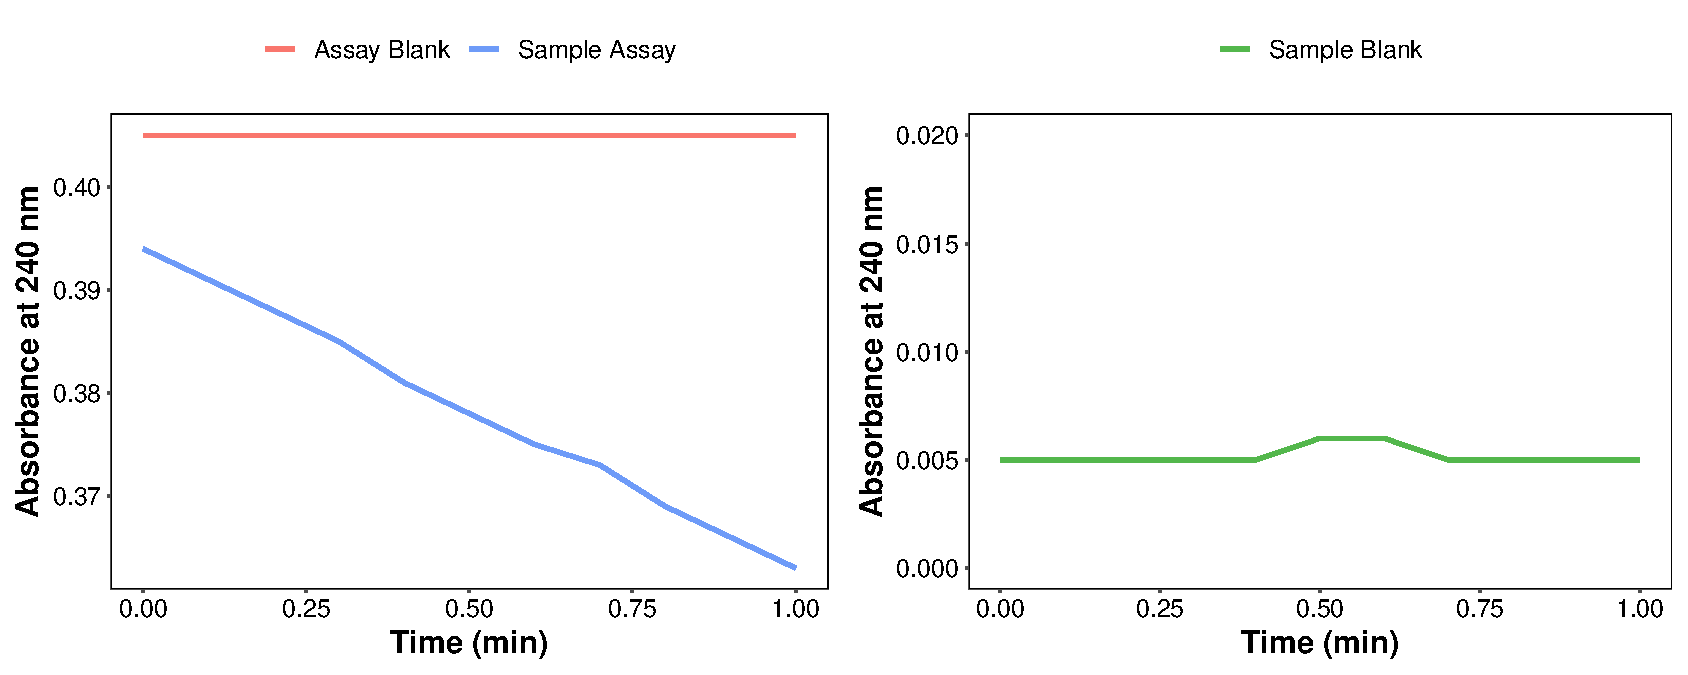
\includegraphics[width=1\linewidth]{Volume-1_files/figure-latex/fig-cat-assay-curves-1} 

}

\caption{\textbf{Representative Readings}. Readings illustrating the variation profile of absorbance over the reading time for Assay Blank, Sample Assay, and Sample Blank. For both \enquote{blanks,} there is no change in absorbance at 240 nm over time. In the Assay Blank, the absorbance remains at \textasciitilde0.4 (equivalent to 10 mM H\textsubscript{2}O\textsubscript{2}). In the Sample Blank, the absorbance is near zero due to the absence of H\textsubscript{2}O\textsubscript{2}. In the Sample Assay, the absorbance starts near \textasciitilde0.4 (equivalent to 10 mM H\textsubscript{2}O\textsubscript{2}) and falls linearly during the reading time.}\label{fig:fig-cat-assay-curves}
\end{figure}

\normalsize

Using increasing amounts of the sample, it is possible to observe an increase in the rate of hydrogen peroxide consumption, corresponding with the increased amount of catalase in the reaction medium (Figure \ref{fig:fig-cat-smp-vol-curves}). However, beyond a certain sample quantity, the amount of catalase becomes excessive, which is evidenced by the non-linearity of the absorbance decrease at 240 nm during the reading. This can be seen in the readings obtained with sample volumes of 10 and 20 µL in the example below (Figure \ref{fig:fig-cat-smp-vol-curves}).



\scriptsize

\begin{figure}

{\centering 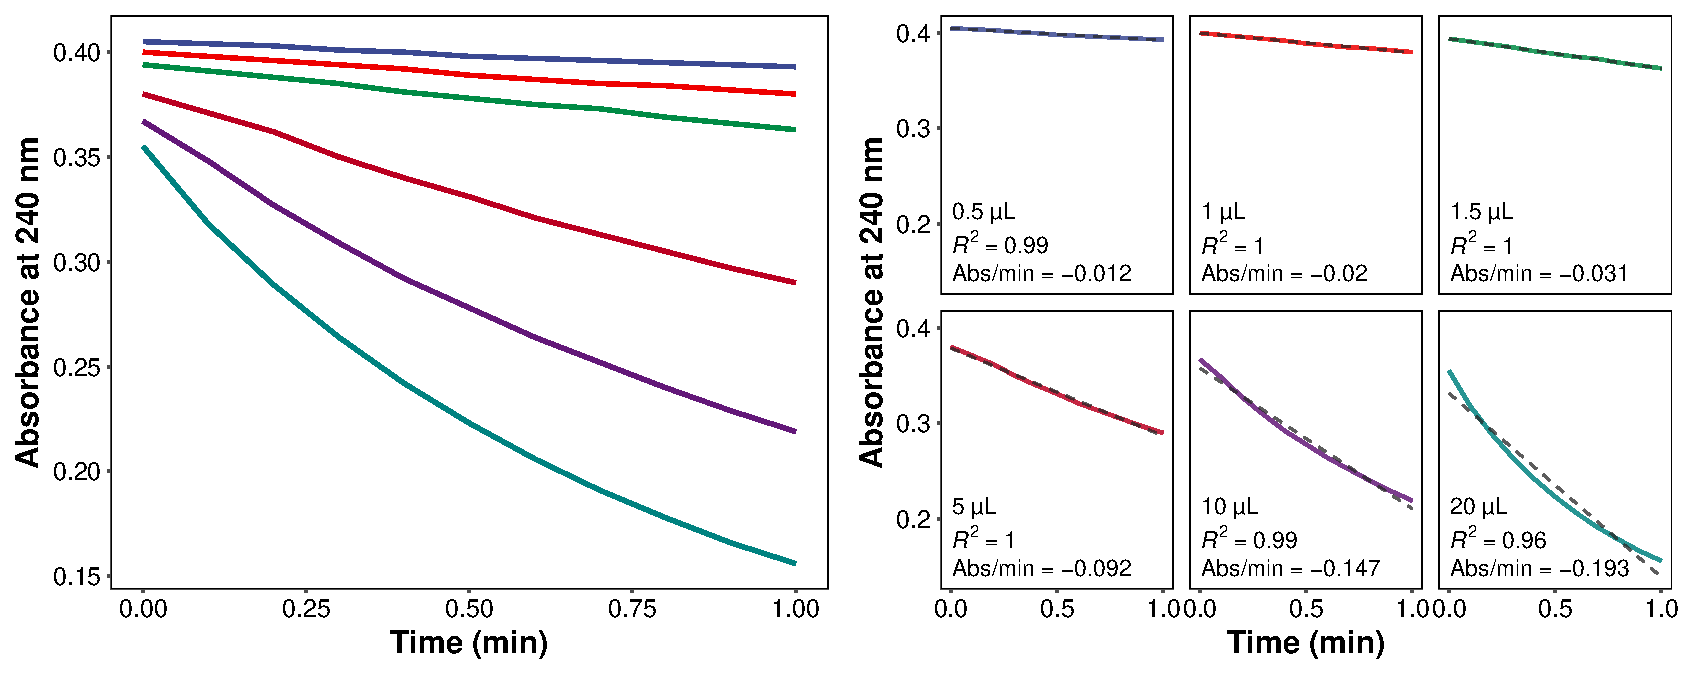
\includegraphics[width=1\linewidth]{Volume-1_files/figure-latex/fig-cat-smp-vol-curves-1} 

}

\caption{\textbf{Sample Assay Readings}. Absorbance decline profiles at 240 nm using different volumes (0.5 - 20 µL) of rat liver homogenate (1:150, w/v). When there is an excess of sample (e.g., ≥ 10 µL), the substrate consumption is so rapid that it causes significant variation in substrate concentration during the reading. This variation affects the enzyme activity during the reading, resulting in a non-linear consumption rate. Note that the initial absorbance differs between the different sample volumes used, as there is consumption of hydrogen peroxide between the time of reagent addition and the start of the reading.}\label{fig:fig-cat-smp-vol-curves}
\end{figure}

\normalsize

Therefore, one should avoid homogenate volumes that result in very high consumption rates, using a sample amount that falls within the linear range of the relationship between rate (Abs/min) and sample quantity. Under the experimental conditions described in this protocol, the rate (Abs/min) \emph{versus} sample quantity relationship is linear up to approximately -0.070 Abs/min (Figure \ref{fig:fig-cat-linear-range}). Nevertheless, it is recommended to use a sample volume that results in a rate between -0.025 and -0.035 for all samples. That is, the volume of each sample should be experimentally determined and adjusted, on a case-by-case basis, to achieve Abs/min values within this range.



\scriptsize

\begin{figure}

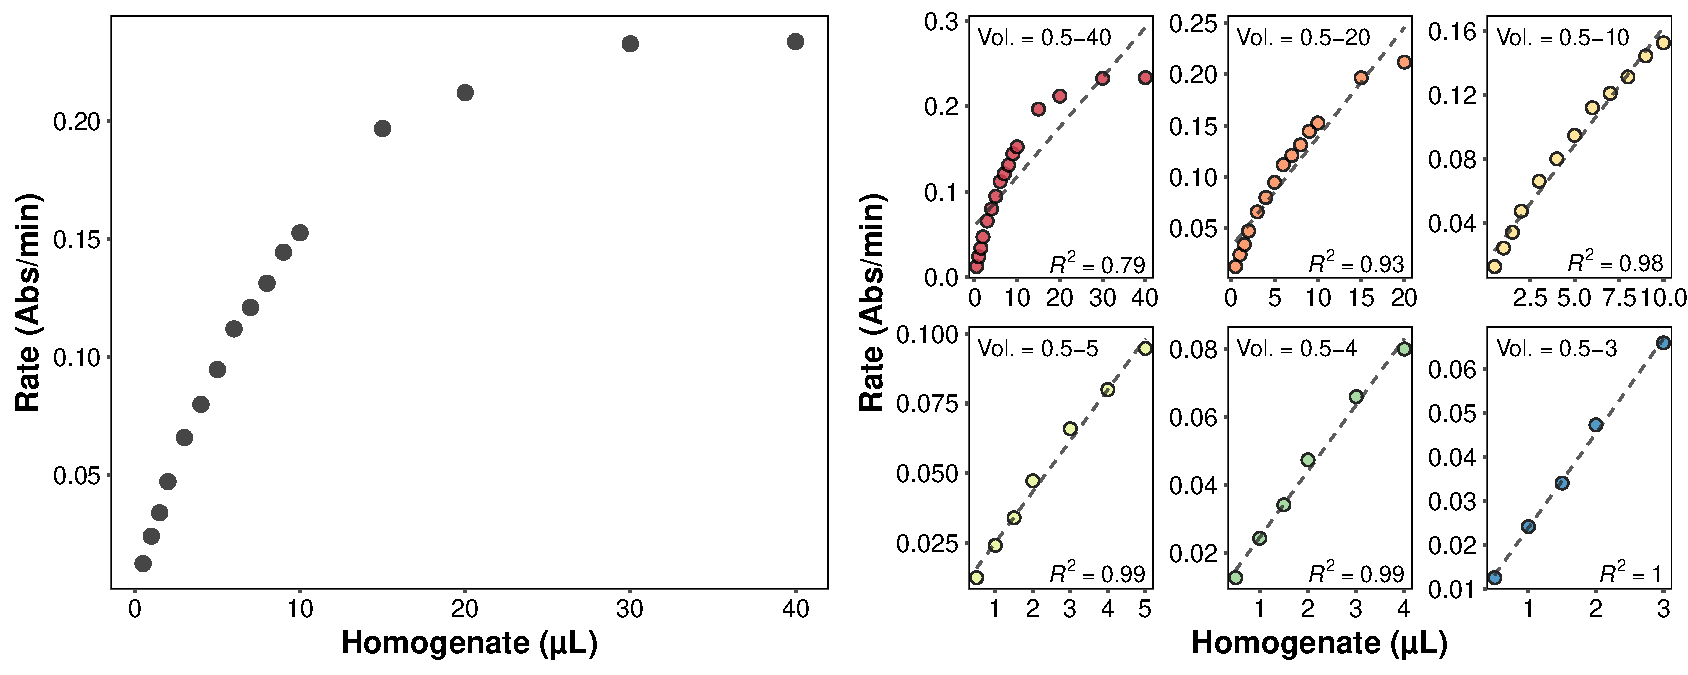
\includegraphics[width=1\linewidth]{Volume-1_files/figure-latex/fig-cat-linear-range-1} \hfill{}

\caption{\textbf{H\textsubscript{2}O\textsubscript{2} Consumption Rate} \emph{versus} \textbf{Sample Quantity}. Different volumes of rat liver homogenate (1:150, w/v) from 0.5 µL to 40 µL were added in the assay to determine catalase activity. The relationship between Abs/min and sample quantity is linear up to a point where the consumption of H\textsubscript{2}O\textsubscript{2} no longer proportionally corresponds to the amount of sample.}\label{fig:fig-cat-linear-range}
\end{figure}

\normalsize

\section{Calculations}\label{calculations}

Enzymatic activity is often expressed in units per volume (U/mL) or mass (U/mg). An enzyme activity unit (U) is defined as the amount of enzyme that catalyzes the consumption of one micromole of substrate per minute (1 U = µmol/min). In enzymatic assays where the formation of a reaction product is monitored, the unit is defined as the amount of enzyme that catalyzes the production of one micromole of product per minute.

To calculate the activity of catalase in U, we use the formula:

\[ 
\text{Activity (U/mL)} = \left( \frac{\Delta \text{Abs}_{240}/\text{min}}{\varepsilon} \right) \times \text{Dilution 1} \times \text{Dilution 2} \times \text{Dilution 3}
\]

where \(\Delta \text{Abs}_{240}/\text{min}\) is the change in absorbance at 240 nm per minute (i.e., the rate); \(\varepsilon\) is the molar absorptivity coefficient; \(\text{Dilution 1}\) is the dilution factor performed in the assay; \(\text{Dilution 2}\) is the dilution factor performed in the sample preparation; and \(\text{Dilution 3}\) is the dilution factor of any other dilution performed.

Note that we are using units per milliliter (U/mL), as, considering that absorbance values are unitless (\(\text{Absorbance} = \log_{10} \left( \frac{I_0}{I} \right)\)) and the readings were performed in a cuvette with an optical path of 1 cm, dividing \(\Delta \text{Abs}_{240}/\text{min}\) by \(\varepsilon\) results in \(\text{U/mL}\):

\[ \frac{\text{cm}^{-1}\text{min}^{-1}}{\text{mM}^{-1}\text{cm}^{-1}} = \text{mM} \cdot \text{min}^{-1} \]

Converting:

\[ \text{mM} \cdot \text{min}^{-1} = \text{mmol/L} \cdot \text{min}^{-1} = \mu\text{mol/mL} \cdot \text{min}^{-1} = \text{U/mL} \]

\begin{greybox}[frametitle = Note]
\emph{Catalase does not follow the usual pattern of Michaelis-Menten kinetics. It is not possible to saturate the enzyme with substrate within a feasible concentration range, and catalase is inactivated (oxidized) by its own substrate at concentrations of H\textsubscript{2}O\textsubscript{2} above 100 mM. Therefore, some authors recommend not using the International Unit to express catalase activity, but rather the rate constant of a first-order reaction (\(k\).}

\end{greybox}

\subsection{Example Calculation}\label{example-calculation}

The steps to calculate the enzymatic activity of catalase in U include calculating the average Abs\textsubscript{240}/min from technical replicates of the sample assay, correcting the average Abs\textsubscript{240}/min by the average value from technical replicates of the sample blank, calculating the activity in the reaction medium, adjusting for the dilution performed in the assay, and the final adjustment for the initial dilution of the tissue in the preparation of the homogenate.

\subsubsection{\texorpdfstring{Mean Abs\textsubscript{240}/min and Correction by Blank}{Mean Abs240/min and Correction by Blank}}\label{mean-abs240min-and-correction-by-blank}

First, calculate the mean of the Abs\textsubscript{240}/min values recorded for the sample blank and the sample assay. Then, subtract the average value of the sample blank from the average value of the sample assay:

\[ \Delta \text{Abs}_{240}/\text{min} = \left( \frac{Assay 1 + Assay 2 + Assay 3}{3} \right) - \left( \frac{Blank 1 + Blank 2 + Blank 3}{3} \right)
\]

Assuming that a sample resulted in rates of -0.0001, 0.0002, -0.0001 for the sample blank, and -0.03, -0.028, -0.032 for the sample assay, we have:

\[ \Delta \text{Abs}_{240}/\text{min} = \left( \frac{-0.03 + -0.028 + -0.032}{3} \right) - \left( \frac{-0.0001 + 0.0002 + -0.0001}{3} \right)\]

\[ \Delta \text{Abs}_{240}/\text{min} = (-0.03) - (0)
\]

\[ \Delta \text{Abs}_{240}/\text{min} = -0.03
\]

\begin{greybox}[frametitle = Note]
\emph{From this point onward, it is advisable to use the absolute value of the change in absorbance ΔAbs/min (i.e., consider the magnitude without regard to its sign). The sign is negative in this protocol because the molecule being monitored is consumed during the assay, causing a decrease in absorbance over time.}

\end{greybox}

\subsubsection{Activity in the Reaction Medium}\label{activity-in-the-reaction-medium}

The corrected average value is divided by the molar absorptivity coefficient of H\textsubscript{2}O\textsubscript{2} at 240 nm (ε\textsubscript{240} = 0.0394 mM\textsuperscript{-1} cm\textsuperscript{-1}) to calculate the activity of catalase in the assay's reaction medium (i.e., the amount of enzyme in the cuvette):

\[ \text{Activity (U/mL) in cuvette} = \left( \frac{0.03}{0.0394} \right) \]

\[ \text{Activity (U/mL) in cuvette} = 0.761\]

\subsubsection{Activity in the Homogenate}\label{activity-in-the-homogenate}

To determine the activity of catalase in the homogenate, multiply the activity in the reaction medium by the dilution factor used in the assay (i.e., the final volume of the assay divided by the volume of sample added). For example, if 20 µL of homogenate were added to a final volume of 800 µL, we have a dilution factor of 40:

\[ \text{Activity (U/mL) in homogenate} = 0.761 \times \left( \frac{800}{20} \right)\]
\[ \text{Activity (U/mL) in homogenate} = 0.761 \times 40\]
\[ \text{Activity (U/mL) in homogenate} = 30.46 \]

\subsubsection{Activity in Tissue}\label{activity-in-tissue}

To calculate the activity of catalase in the sample, simply multiply the activity value in the homogenate by any dilutions that have been performed up to the point of assay. The preparation of the homogenate always involves an initial dilution at the time of homogenization. Often, after a centrifugation step, the homogenate is diluted again. Therefore, assuming that a homogenate was initially prepared at a ratio of 1:5 (w/v) (e.g., 100 mg of tissue in 500 µL of final volume) and that after homogenization and centrifugation the homogenate was diluted again 1:400 (e.g., 3 µL of supernatant in 1200 µL of final volume), there is a total dilution factor of 2000:

\[ \text{Activity (U/mL) in tissue} = 30.46 \times \left( \frac{500}{100} \right) \times \left( \frac{1200}{3} \right)\]

\[ \text{Activity (U/mL) in tissue} = 30.46 \times 5 \times 400\]

\[ \text{Activity (U/mL) in tissue} = 30.46 \times 2000\]

\[ \text{Activity (U/gww) in tissue} = 60913.71\]

\begin{greybox}[frametitle = Note]
\emph{Here, catalase activity is expressed in units per gram of wet weight tissue (U/gww). It is assumed that the density of water (1 g/mL) is an acceptable approximation for the density of biological tissues. If this approximation is not suitable for the sample or tissue being analyzed, catalase activity can be normalized by protein concentration at any of the previous steps, whether in the reaction medium activity or in the homogenate.}

\end{greybox}

\subsubsection{Normalization by Protein Concentration}\label{normalization-by-protein-concentration}

Lastly, to standardize the comparison of enzymatic activity across different samples and experiments, enzymatic activity values are commonly normalized by the amount of protein in the sample. This is done by dividing the calculated activity (U/gww) by the protein concentration in the sample (mg prot./gww). Normalization can be done at any previous step if the protein concentration in the reaction medium or homogenate is known. Assuming that the sample has a protein concentration of 99.1 mg/gww, we have:

\[ \text{Activity (U/mg prot.) in tissue} = \left( \frac{\ensuremath{6.091371\times 10^{4}}}{99.1} \right)\]
\[ \text{Activity (U/mg prot.) in tissue} = 614.67 \]

\begin{greybox}[frametitle = Note]
\emph{To normalize enzymatic activity, it is necessary to quantify the protein concentration in the sample using another method (e.g., Bradford assay, BCA, Qubit™, etc.). Quantification should be done using the same homogenate used to measure activity.}

\end{greybox}

\section{3-Amino-1,2,4-Triazole}\label{amino-124-triazole}

To ensure that the consumption of H\textsubscript{2}O\textsubscript{2} observed in the assay is specifically caused by catalase activity, it is recommended to verify the ability of 3-amino-1,2,4-triazole (ATZ) to reduce the rate of H\textsubscript{2}O\textsubscript{2} consumption caused by the sample. ATZ is an irreversible inhibitor of catalase and is used at a concentration of 20 mM with an exposure time of 0.5 to 2.0 hours to abolish catalase activity \autocite{margoliash_study_1958,margoliash_irreversible_1960,watanabe_autoxidation_2003}. Since ATZ acts on Compound I (see \hyperref[intro]{Introduction}), and not directly on catalase, H\textsubscript{2}O\textsubscript{2} should be added to the medium where the sample is incubated with ATZ so that Compound I is formed and inhibition occurs.

\subsection{\texorpdfstring{Catalase Inhibition by ATZ \emph{in vitro}}{Catalase Inhibition by ATZ in vitro}}\label{catalase-inhibition-by-atz-in-vitro}

The following result illustrates the effect of incubating a sample with ATZ in the absence and presence of H\textsubscript{2}O\textsubscript{2}. Aliquots of rat liver homogenate were diluted in PBS (resulting in a catalase activity of 40.61 U/mL) and incubated at 22°C for 2.5 hours under three conditions: in the absence of any inhibitor (control), in the presence of 20 mM ATZ (ATZ), and in the presence of 20 mM ATZ + 4 mM H\textsubscript{2}O\textsubscript{2} (ATZ + H\textsubscript{2}O\textsubscript{2}) (Figure \ref{fig:cat-fig-inhibitor}). As the catalase present in the sample consumes H\textsubscript{2}O\textsubscript{2} over time, the reaction medium of the ATZ + H\textsubscript{2}O\textsubscript{2} treatment was supplemented with H\textsubscript{2}O\textsubscript{2} at 0.5-hour intervals to maintain a concentration of 4 mM during the incubation. For the control and ATZ groups, the same volumes of PBS were added to ensure the same dilution factor between treatments.



\scriptsize

\begin{figure}

{\centering 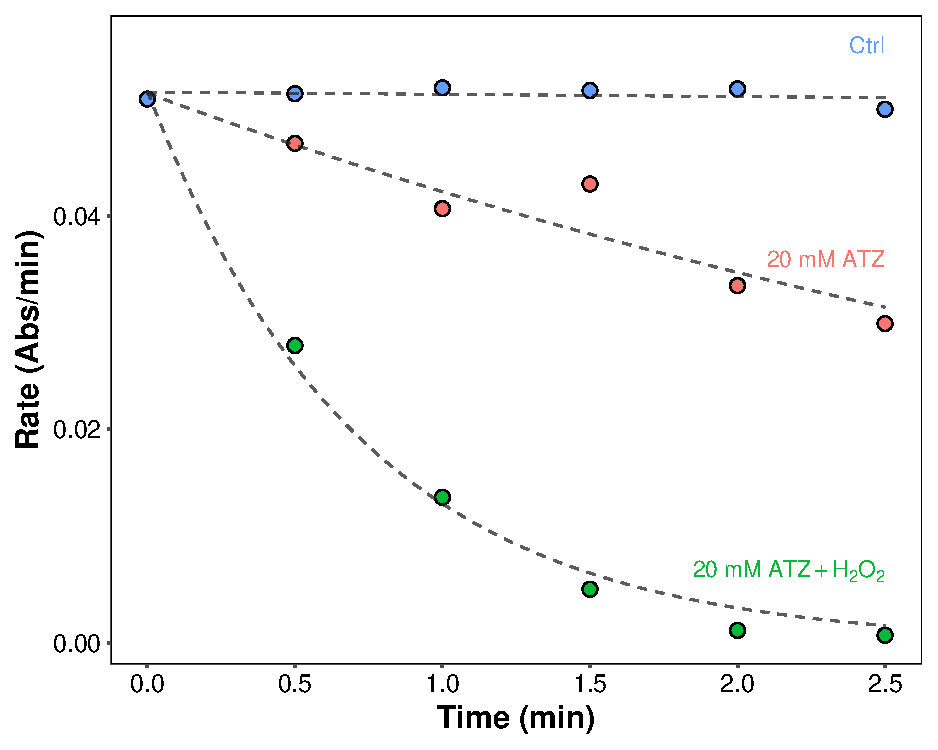
\includegraphics[width=0.5\linewidth]{Volume-1_files/figure-latex/cat-fig-inhibitor-1} 

}

\caption{\textbf{Inhibition of catalase activity by 3-amino-1,2,4-triazole (ATZ)}. Effect of incubating samples of rat liver homogenate with 20 mM ATZ in the absence and presence of 4 mM H\textsubscript{2}O\textsubscript{2} over 2.5 hours. The samples were diluted in PBS, resulting in a catalase activity of 40.61 U/mL, and incubated at 22°C under three different conditions: control (no inhibitors), presence of 20 mM ATZ, and presence of 20 mM ATZ + 4 mM H\textsubscript{2}O\textsubscript{2}. During the incubation, the reaction medium of the ATZ + H\textsubscript{2}O\textsubscript{2} treatment was supplemented with H\textsubscript{2}O\textsubscript{2} every 0.5 hours to maintain a constant concentration of 4 mM. In the control and ATZ treatments, equivalent volumes of PBS were added to maintain the same dilution factor.}\label{fig:cat-fig-inhibitor}
\end{figure}

\normalsize

In the control treatment, catalase activity remained stable throughout the period, oscillating between -0.050 and -0.052 Abs/min. In the ATZ treatment, catalase activity gradually declined, but after 2.5 hours, the inhibition was only 41.3\% relative to the initial activity. In the sample treated with ATZ + H\textsubscript{2}O\textsubscript{2}, the activity dropped exponentially, being only 1.5\% of the control treatment and the initial activity before the start of the treatment (\hyperref[fig-inhibitor]{Figure 4}). Therefore, for this sample, all consumption of H\textsubscript{2}O\textsubscript{2} can be attributed to catalase activity.

\section{Troubleshooting}\label{troubleshooting}

It has been reported that for some species there is a delay for the onset of h2o2 consumption.

When optimizing the assay or assessing no a sample for the first time it is better to use longer total reading time to better understand what is going on and diagnose potential problems.

\scriptsize

\begin{table}[!h]
\centering
\caption{\label{tab:cat-troubleshooting}caption}
\centering
\fontsize{7}{9}\selectfont
\begin{tabular}[t]{>{\raggedright\arraybackslash}p{15em}>{\raggedright\arraybackslash}p{10em}>{\raggedright\arraybackslash}p{15em}}
\toprule
\textbf{Problem} & \textbf{Possible Cause} & \textbf{Solution}\\
\midrule
\cellcolor{gray!10}{Inconsistent results between runs} & \cellcolor{gray!10}{Pipetting errors} & \cellcolor{gray!10}{Calibrate pipettes and ensure consistent technique}\\
 & Temperature variations & Maintain a consistent temperature environment during the experiment\\
\cellcolor{gray!10}{} & \cellcolor{gray!10}{Inconsistent incubation times} & \cellcolor{gray!10}{Standardize and carefully monitor incubation times}\\
No change in absorbance over time & Incorrect wavelength selected & Verify and set the correct wavelength\\
\cellcolor{gray!10}{} & \cellcolor{gray!10}{Sample not added} & \cellcolor{gray!10}{Ensure the sample is correctly pipetted into the wells}\\
\addlinespace
High initial absorbance &  & \\
\cellcolor{gray!10}{Low initial absorbance} & \cellcolor{gray!10}{} & \cellcolor{gray!10}{}\\
Non-linear rate &  & \\
\bottomrule
\end{tabular}
\end{table}

\normalsize

\section{Additional Comments}\label{cat_additional_comments}



\subsection{Catalase}\label{catalase-1}

\begin{itemize}
\tightlist
\item
  \textbf{Hydrogen Peroxide Concentration}: A concentration of 10 mM H\textsubscript{2}O\textsubscript{2} is used to prevent enzyme inactivation during the assay and to minimize the formation of bubbles (O\textsubscript{2}) inside the cuvette. Since the concentration of H\textsubscript{2}O\textsubscript{2} is critical and at 10 mM the enzyme is not saturated (Figure \ref{fig:fig-substrate-curves}), it is essential to always check the stock solution concentration before each assay (see \hyperref[checking_h2o2]{Hydrogen Peroxide (H\textsubscript{2}O\textsubscript{2})}) and ensure that sample readings start with absorbance values close to 0.4.
\end{itemize}

\scriptsize

\begin{figure}\setbox0=\hbox{\begin{minipage}[h]{\widthw}\centering 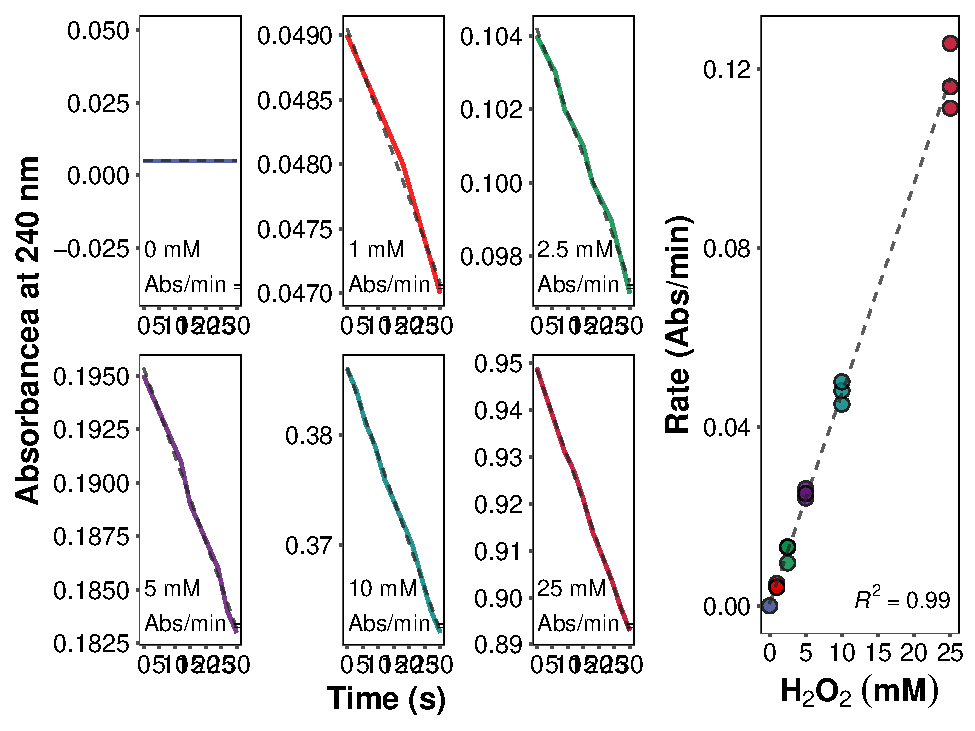
\includegraphics[width=\widthw]{Volume-1_files/figure-latex/fig-substrate-curves-1} \end{minipage}}\needspace{\ht0+\dp0+2\baselineskip}\definesHSpace\hspace{-\rf}\box0\caption{\textbf{Rate of H\textsubscript{2}O\textsubscript{2} Consumption} \emph{versus} \textbf{Substrate Concentration}. Effect of the final concentration of H\textsubscript{2}O\textsubscript{2} on the assay for determining catalase activity. The left panel shows representative readings from assays with final concentrations of 1, 2.5, 5, 10, and 25 mM of H\textsubscript{2}O\textsubscript{2}, in addition to the control in the absence of H\textsubscript{2}O\textsubscript{2}. Note that at the concentration of 25 mM, the absorbance approaches 1 in a cuvette with a 1 cm optical path. The reading time was reduced to 30 seconds to allow comparison between concentrations, as at 25 mM of H\textsubscript{2}O\textsubscript{2}, the Abs/min rate ceases to be linear after 30 seconds under the conditions of the experiment. The right-hand chart shows a linear relationship between substrate concentration and enzymatic activity, indicating that the enzyme is not saturated within this concentration range. The chart displays data from three different readings for each concentration of H\textsubscript{2}O\textsubscript{2}.}\label{fig:fig-substrate-curves}
\end{figure}

\normalsize

\begin{itemize}
\item
  \textbf{Temperature}: Temperature has a minimal effect on catalase activity (Q\textsubscript{10} ≈ 1.1). Therefore, measurements can be performed over a wide range of temperatures (e.g., 10°C to 37°C) without significant variation (\href{https://doi.org/10.1016/S0076-6879(84)05016-3}{Aebi 1984}). Nonetheless, it is recommended to conduct assays at a consistent temperature (e.g., 25°C or another physiologically relevant temperature for the sample) for samples that will be compared with each other.
\item
  \textbf{Optimal pH}: Catalase has optimal activity in a pH range of 6.8-7.5 (\href{https://doi.org/10.1016/S0076-6879(84)05016-3}{Aebi 1984}).
\item
  \textbf{Bubble Formation}: The formation of bubbles during the assay reading of a sample (\hyperref[fig-catalase-bubbles]{Figure 6}) is an indicator that there is an excess of catalase in the assay and that the reading should be repeated with a smaller sample volume. In addition to indicating excessive substrate consumption, bubbles generate noise in absorbance measurements.
\end{itemize}



\scriptsize

\begin{figure}\setbox0=\hbox{\begin{minipage}[h]{\widthw}\centering 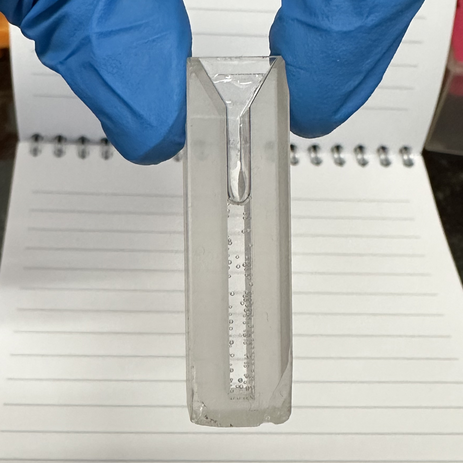
\includegraphics[width=\widthw]{images/catalase/bubbles} \end{minipage}}\needspace{\ht0+\dp0+2\baselineskip}\definesHSpace\hspace{-\rf}\box0\caption{\textbf{Bubble Formation}. Formation of bubbles (O\textsubscript{2}) inside the cuvette after a 1-minute reading. The recorded Abs\textsubscript{240}/min value in this reading was -0.150.}\label{fig:fig-cat-bubbles}
\end{figure}

\normalsize

\begin{itemize}
\tightlist
\item
  \textbf{Minimizing Pre-Reading H\textsubscript{2}O\textsubscript{2} Consumption}: A strategy to minimize the consumption of H\textsubscript{2}O\textsubscript{2} between the addition of the sample and the actual start of the reading is to use a piece of Parafilm to position a small volume of sample (≤ 5 µL). Cover the cuvette with the Parafilm without moving the droplet (Figure \ref{fig:fig-catalase-parafilm}), invert the cuvette to homogenize the contents, place it in the cuvette holder, and start the reading. This way, the interval between the first contact of the sample with the reaction medium and the start of the reading is minimized, ensuring that the reading actually begins with the final assay concentration of 10 mM H\textsubscript{2}O\textsubscript{2}.
\end{itemize}



\scriptsize

\begin{figure}\setbox0=\hbox{\begin{minipage}[h]{\widthw}\centering 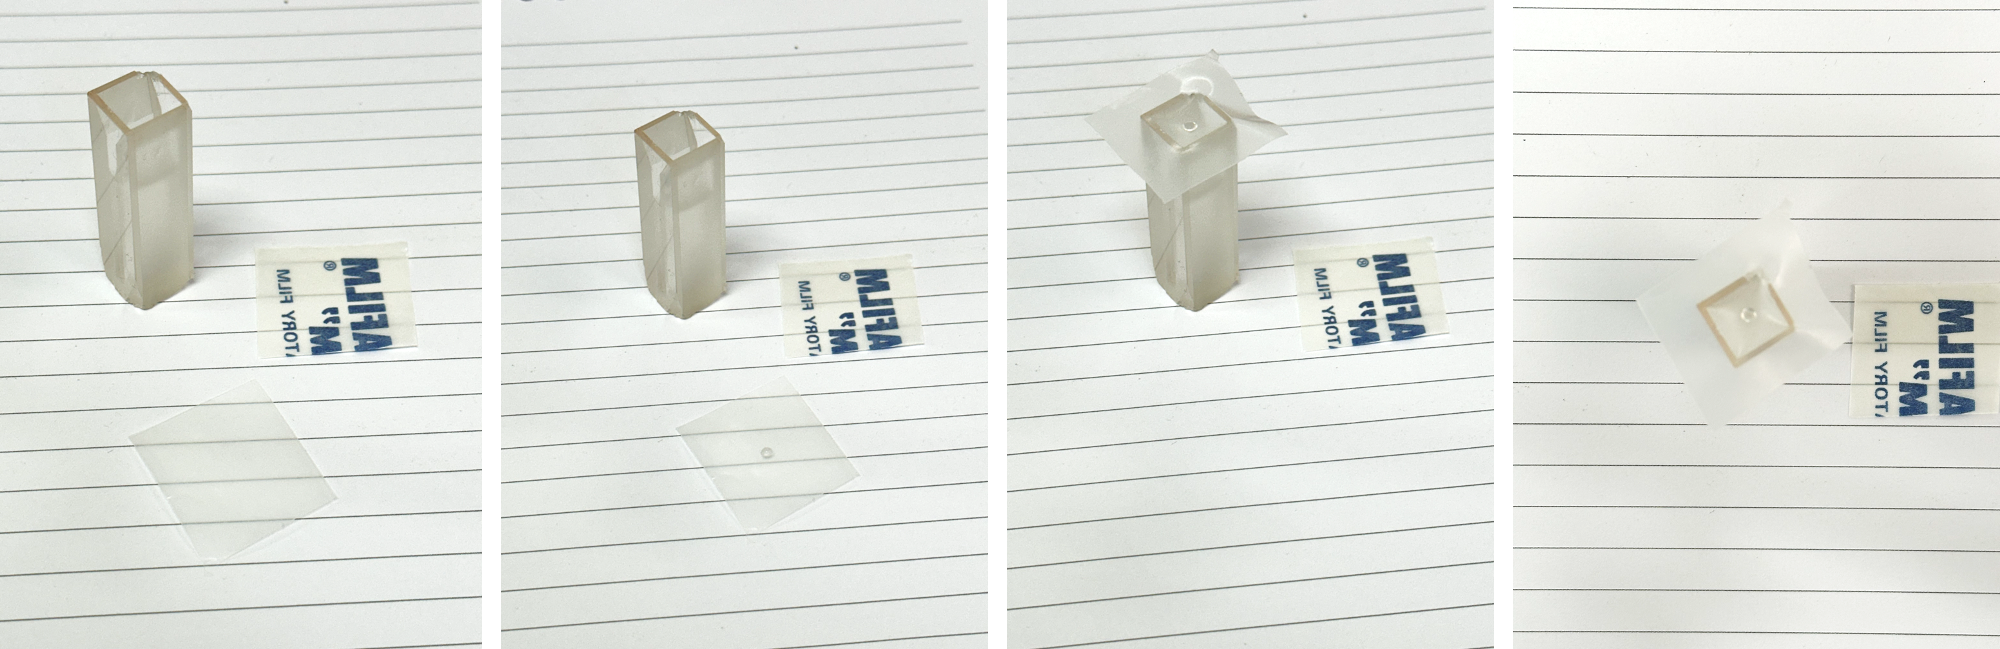
\includegraphics[width=\widthw]{images/catalase/parafilm_droplet} \end{minipage}}\needspace{\ht0+\dp0+2\baselineskip}\definesHSpace\hspace{-\rf}\box0\caption{\textbf{Minimizing Pre-Reading H\textsubscript{2}O\textsubscript{2} Consumption}. Steps to ensure rapid initiation of the reading after the sample contacts the reaction medium of the assay. This procedure minimizes the consumption of H\textsubscript{2}O\textsubscript{2} before the start of the reading, which is crucial in the absence of automatic injection and mixing systems. Add a volume of up to 5 µL of sample on a piece of Parafilm; carefully cover the cuvette containing buffer, water, and H\textsubscript{2}O\textsubscript{2}; invert the cuvette to homogenize the contents; place it in the holder and start the reading.}\label{fig:fig-cat-parafilm}
\end{figure}

\normalsize

\subsection{Enzymatic Assays}\label{enzymatic-assays}

\begin{itemize}
\item
  \textbf{Temperature Control}: Like common chemical reactions, temperature significantly affects the speed of enzymatic reactions. For most enzyme-catalyzed reactions, the rate increases 2-3 times with every 10°C increase (temperature coefficient, Q\textsubscript{10} = 2-3). That is, an increase in temperature within a specific range accelerates the reaction. To ensure the comparability of results from different samples and experimental days, readings should be made at the same temperature, preferably one that is physiologically relevant to the organism of origin (e.g., 37°C for human tissues). Microplate readers and spectrophotometers have temperature control systems for this purpose. Additionally, it is recommended to keep the deionized water used in the protocol at the assay temperature (e.g., using a water bath or dry block heaters). As most of the reaction medium volume is composed of water, ensuring the water is at the correct temperature helps stabilize the temperature of the reaction medium more quickly.
\item
  \textbf{pH Control}: Enzymes are sensitive to pH variations and have an optimum pH at which their catalytic activity is maximized. The relationship between enzymatic activity and pH is a bell-shaped curve, with the peak indicating the optimum pH. From the optimum pH, towards alkaline or acidic extremes, the activity of the enzyme decreases as the pH changes until it finally reaches zero at the extremes. This is because pH affects the ionization of charged groups involved in the catalytic mechanism and/or structural stability of the enzyme. Generally, enzymatic assays are conducted at physiological pH for the organism from which the sample originates. However, in some cases, it is convenient to use a pH that differs from the physiological for analytical reasons.
\item
  \textbf{Substrate Concentration}: Ideally, saturating concentrations of substrates and cofactors should always be used to determine an enzyme's activity. However, factors such as high molar absorptivity and low solubility prevent the assay from being conducted at such concentrations in most cases.
\item
  \textbf{Initial Rate vs.~V\textsubscript{max}}: Although some equipment expresses the initial change in absorbance over time (representing the change in substrate or product concentration) in an enzymatic assay as V\textsubscript{max}, this value is actually the initial rate (v\textsubscript{0}). Note that V\textsubscript{max} is a theoretical limit never reached in any experiment, although it is possible to approach it and determine it by extrapolation. This limitation is caused by the fact that complete saturation can only be achieved at infinite concentrations of substrates and cofactors, and, despite using high concentrations of substrates and cofactors, the concentrations cannot be considered as completely saturating.
\item
  \textbf{Enzyme Unit}: The enzyme unit, or international unit of enzymatic activity (U, sometimes IU), is a measure of an enzyme's catalytic activity. This unit is defined as the amount of enzyme that catalyzes the conversion of one µmol of substrate per minute (1 U = µmol/min), under conditions specified by the assay method.
\item
  \textbf{Expression of Enzymatic Activity}: Measures of enzymatic activity are often expressed as units per milligram of protein (U/mg protein), both in cell lysates or tissue homogenates and in isolated protein preparations. This practice is based on the need to normalize enzymatic activity relative to the amount of protein present in the sample, providing a standardized way to compare enzymatic activity between different samples and experiments.
\end{itemize}

\subsection{General Observations}\label{general-observations}

\begin{itemize}
\item
  \textbf{Volume Adjustments and Optical Path Length}: The final volume and the volumes of reagents can be adjusted for stock solutions of different concentrations and reading containers of different volumes, such as cuvettes or microplates, provided that the final concentrations are maintained as specified in the protocol. It is crucial to adjust the obtained signal for an optical path length of 1 cm, as the molar coefficient indicated in the protocol is in cm\textsuperscript{-1}. This means that if a reading container with a different optical path length is used, the absorbance value should be multiplied by the ratio between 1 cm and the new path length, ensuring the correct adjustment of the measured signal. For example, if the optical path is 0.5 cm, the measured absorbance should be multiplied by 2.
\item
  \textbf{Useful Formulas}: The following formulas are useful for verifying protocol information or adjusting the quantity/volume of the solution, as needed on a case-by-case basis. For all of them, it is important to pay attention to the units of each variable.

  \begin{itemize}
  \tightlist
  \item
    To prepare dilutions from stock solutions: \(C_1 \cdot V_1 = C_2 \cdot V_2\)
  \item
    To prepare a new solution from volume and concentration or mass and concentration: \(\text{Mass (g)} = \text{Concentration (M)} \cdot \text{Volume (L)} \cdot \text{Molecular Weight (g/mol)}\)
  \item
    Lambert-Beer Law: \(A = \varepsilon \cdot C \cdot l\), where \(A\) is absorbance; \(\varepsilon\) is the molar absorption coefficient (M\textsuperscript{-1} cm\textsuperscript{-1}); \(C\) is the concentration of the solution (M); \(l\) is the path length of the optical path (cm).
  \end{itemize}
\end{itemize}

\chapter{Superoxide Dismutase}\label{superoxide-dismutase}


% Bibliography
%%%%%%%%%%%%%%%%%%%%%%%%%%%%%%%%%%%%%%%%%%%%%%%%%%%%%%%%%%

\backmatter
\SmallMargins

\printbibliography
\onecolumn


% Tables (of tables, of figures)
%%%%%%%%%%%%%%%%%%%%%%%%%%%%%%%%%%%%%%%%%%%%%%%%%%%%%%%%%%




% After-body (LaTeX code inclusion)
%%%%%%%%%%%%%%%%%%%%%%%%%%%%%%%%%%%%%%%%%%%%%%%%%%%%%%%%%%




% Back cover
%%%%%%%%%%%%%%%%%%%%%%%%%%%%%%%%%%%%%%%%%%%%%%%%%%%%%%%%%%%

% Even page, small margins, no running head, no page number.
\evenpage
\SmallMargins
\thispagestyle{empty}

\begin{normalsize}

\begin{description}

\selectlanguage{english}
\item[Abstract]
English abstract, on the last page. English abstract, on the last page.English abstract, on the last page.English abstract, on the last page.English abstract, on the last page.English abstract, on the last page.English abstract, on the last page.English abstract, on the last page.English abstract, on the last page.English abstract, on the last page.English abstract, on the last page.English abstract, on the last page.
\item[Keywords]
Keyword1, Keyword2, Keyword3, Keyword4, Keyword5.
~\\

\end{description}

\end{normalsize}

\vspace*{\fill}
\centering\includegraphics[width=.3\textwidth]{images/logo}

\end{document}
